\documentclass[12pt,a4paper]{report}

% Essential packages
\usepackage[utf8]{inputenc}
\usepackage{graphicx}
\usepackage[colorlinks=true, linkcolor=blue, citecolor=blue, urlcolor=blue]{hyperref}
\usepackage{booktabs}
\usepackage{tabularx}
\usepackage{float}
\usepackage{listings}
\usepackage{xcolor}
\usepackage{tikz}
\usepackage{pgf-umlcd}
\usepackage{pgf-umlsd}
\usepackage{algorithm}
\usepackage{algpseudocode}
\usepackage{minted}
\usepackage{fancyhdr}
\usepackage{titlesec}
\usepackage{appendix}
\usepackage{geometry}
\usepackage{longtable}
\usepackage{enumitem}
\usepackage{amsmath}
\usepackage{setspace}

% Page setup
\geometry{margin=1in}
\onehalfspacing

% Header and footer
\pagestyle{fancy}
\fancyhf{}
\rhead{\thepage}
\lhead{Campus Placement Management System}
\cfoot{Confidential}

% Title formatting
\titleformat{\chapter}[display]
{\normalfont\huge\bfseries}{\chaptertitlename\ \thechapter}{20pt}{\Huge}
\titlespacing*{\chapter}{0pt}{50pt}{40pt}

% Code listing styling
\definecolor{codegray}{gray}{0.9}
\definecolor{codecomment}{rgb}{0.0,0.5,0.0}
\definecolor{codestring}{rgb}{0.6,0.1,0.1}

\lstset{
    backgroundcolor=\color{codegray},
    commentstyle=\color{codecomment},
    stringstyle=\color{codestring},
    basicstyle=\ttfamily\small,
    breaklines=true,
    captionpos=b,
    keepspaces=true,
    numbersep=5pt,
    showspaces=false,
    showstringspaces=false,
    showtabs=false,
    tabsize=2
}

% Document information
\title{
    \vspace{-1.5cm}
    \LARGE \textbf{Campus Placement Management System}\\
    \vspace{0.5cm}
    \large Comprehensive Analysis, Design, Implementation, and Evaluation\\
    \vspace{1.5cm}
    \includegraphics[width=0.4\textwidth]{project_logo.png}\\
    \vspace{1.5cm}
}
\author{
    \textbf{Prepared by:}\\
    University Institute of Technology\\
    \texttt{placement-team@university.edu}\\
    \vspace{0.5cm}
    \textbf{Organization:}\\
    University Institute of Technology\\
    Department of Computer Science
}
\date{\today}

\begin{document}

% Title page
\maketitle
\thispagestyle{empty}

% Executive Summary
\begin{abstract}
    \begin{center}
        \large\textbf{Executive Summary}
    \end{center}
    This comprehensive report presents a detailed analysis and documentation of the Campus Placement Management System. The project aims to streamline and digitize the campus placement process through the implementation of a full-stack web application using the MERN (MongoDB, Express.js, React.js, Node.js) stack. The system architecture follows a modern single-page application approach with a RESTful API backend to ensure scalability, maintainability, and security.
    
    Key achievements of this project include the development of a multi-role access system with specialized interfaces for students and administrators, implementation of a comprehensive application tracking system, a real-time notification framework, a department-based student organization system, and a detailed reporting dashboard for placement statistics. Performance testing demonstrates excellent response times under normal load and acceptable degradation during peak usage periods. The implemented solution successfully addresses the requirements specified by stakeholders and provides a foundation for future enhancements.
    
    This document contains detailed workflows, database schemas, system architecture diagrams, implementation specifics, and evaluation results. The report concludes with recommendations for future development and potential extensions to the current system, including AI-based candidate matching, enhanced analytics capabilities, and integration with external job portals.
\end{abstract}

% Table of contents and lists
\tableofcontents
\listoffigures
\listoftables
\newpage

% Main content
\chapter{Introduction}
\section{Project Overview}
The Campus Placement Management System is a comprehensive web application designed to streamline and digitize the entire campus placement process for educational institutions. This project addresses the critical need for an organized, efficient, and transparent system to manage the complex interactions between students, placement administrators, and recruiting companies.

The system serves as a centralized platform that connects students seeking employment opportunities with companies looking to recruit talent. It manages the end-to-end placement process, from company registration and job listing to student applications, interview scheduling, and final placement tracking. The platform is particularly notable for its department-based organization system, which efficiently manages students across different academic disciplines (CE, CSE, IT, SFE, ME, EEE, EC).

Built on the MERN (MongoDB, Express.js, React.js, Node.js) stack, the application leverages modern web technologies to deliver a responsive, secure, and scalable solution. MongoDB's document-based architecture provides the flexibility needed to store varied student profiles and application data, while React.js enables a dynamic and interactive user interface. The Express.js/Node.js backend implements robust business logic, authentication, and data processing capabilities.

Key features of the system include:
\begin{itemize}
    \item Secure role-based access control for students and administrators
    \item Comprehensive student profile management with academic and professional details
    \item Department-specific views and operations for efficient administration
    \item Company and job opportunity management with eligibility filtering
    \item Application tracking system with status updates and notifications
    \item Real-time notification system for important events and updates
    \item Interview scheduling and management
    \item Reporting and analytics dashboard for placement statistics
\end{itemize}

\section{Scope and Objectives}
The scope of this project encompasses:
\begin{itemize}
    \item Development of a secure authentication and authorization system with role-based access control (student, admin)
    \item Implementation of student profile management with academic and professional information
    \item Creation of a department-based student organization system (CE, CSE, IT, SFE, ME, EEE, EC)
    \item Design of a company management module for administrators to track recruiting organizations
    \item Development of a job listing and application system with eligibility filtering
    \item Implementation of an application tracking system with status updates and notifications
    \item Creation of an interview scheduling and management system
    \item Development of a real-time notification framework for system events
    \item Implementation of reporting and analytics capabilities for placement statistics
    \item Design of responsive interfaces for both student and admin users
\end{itemize}

The key objectives of this project are:
\begin{enumerate}
    \item To digitize and streamline the manual placement process, reducing administrative overhead by at least 50\%
    \item To improve communication between students, placement administrators, and companies through a centralized platform
    \item To enhance student experience during the placement season with real-time updates and transparent processes
    \item To provide administrators with tools for efficient management of the placement process
    \item To generate actionable insights through analytics to improve placement strategies
    \item To create a scalable system that can accommodate growing numbers of students and companies
    \item To ensure data security and privacy for sensitive student and company information
    \item To create a platform that is accessible across devices through responsive design
\end{enumerate}

\section{Stakeholders}
The following stakeholders are involved in this project:
\begin{itemize}
    \item \textbf{Students:} Primary users who utilize the system to create and maintain their profiles, discover job opportunities, submit applications, and track their progress through the recruitment process. The system provides them with timely notifications, a transparent view of the application process, and resources to prepare for interviews.
    
    \item \textbf{Placement Administrators:} Staff responsible for managing the entire placement process. They use the system to coordinate with companies, manage student eligibility, review applications, schedule interviews, and generate comprehensive reports on placement activities.
    
    \item \textbf{Department Coordinators:} Faculty members who oversee placement activities for specific academic departments (CE, CSE, IT, SFE, ME, EEE, EC). They need department-specific views of student data and placement statistics to ensure their students are effectively represented in the recruitment process.
    
    \item \textbf{Companies/Recruiters:} Organizations looking to hire students. While they interact with the system indirectly through the placement office, their requirements, job descriptions, and recruitment schedules are managed within the platform.
    
    \item \textbf{University Management:} Higher officials who use placement statistics and reports for institutional assessment and strategic planning. They require aggregate data on placement outcomes across departments and academic years.
    
    \item \textbf{IT Support Team:} Technical staff responsible for maintaining the system, ensuring its availability, security, and performance throughout the placement season.
\end{itemize}

\section{Document Structure}
This document is organized into eleven chapters:
\begin{itemize}
    \item \textbf{Chapter 1: Introduction} - Provides an overview of the project, its scope, objectives, and stakeholders.
    \item \textbf{Chapter 2: Background and Context} - Discusses the theoretical and practical context of campus placement management and related technologies.
    \item \textbf{Chapter 3: Requirements Analysis} - Details the functional and non-functional requirements that guided the system development.
    \item \textbf{Chapter 4: System Architecture} - Explains the overall system design and architecture, including component breakdowns and technology stack.
    \item \textbf{Chapter 5: Database Design} - Presents the MongoDB document schemas, relationships, and data organization strategies.
    \item \textbf{Chapter 6: Workflow Diagrams} - Illustrates the key system processes including authentication, application processing, and notification workflows.
    \item \textbf{Chapter 7: Implementation Details} - Describes the implementation specifics including code organization, authentication mechanisms, and API design.
    \item \textbf{Chapter 8: User Interface Design} - Showcases the application's interface design, user experience considerations, and responsive layouts.
    \item \textbf{Chapter 9: Testing and Validation} - Outlines the testing methodology and results for various aspects of the system.
    \item \textbf{Chapter 10: Results and Evaluation} - Presents the project outcomes, performance metrics, and stakeholder feedback.
    \item \textbf{Chapter 11: Conclusion and Future Work} - Summarizes the project achievements and suggests potential future enhancements.
\end{itemize}

\chapter{Background and Context}
\section{Theoretical Background}
\subsection{Campus Placement Process}
The campus placement process represents a structured recruitment mechanism where companies visit educational institutions to select students for employment opportunities. This process typically follows a well-defined lifecycle:

\begin{enumerate}
    \item \textbf{Pre-placement Activities:} The placement office initiates relationships with potential recruiting companies, while students prepare their resumes and professional profiles.
    
    \item \textbf{Company Registration:} Interested companies register with the institution, providing details about their organization, job profiles, requirements, and compensation packages.
    
    \item \textbf{Job Announcement:} The placement office announces job opportunities to eligible students based on criteria such as academic performance, department, and specific company requirements.
    
    \item \textbf{Student Application:} Interested and eligible students submit their applications with resumes and other required documents.
    
    \item \textbf{Application Screening:} Companies review applications and select candidates for further assessment.
    
    \item \textbf{Assessment Process:} Selected candidates undergo various assessment rounds, which may include aptitude tests, technical interviews, HR interviews, and group discussions.
    
    \item \textbf{Job Offers:} Successful candidates receive job offers with details of compensation and terms of employment.
    
    \item \textbf{Acceptance/Rejection:} Students decide whether to accept or reject the offers.
    
    \item \textbf{Post-placement Activities:} The placement office compiles statistics, gathers feedback, and prepares reports.
\end{enumerate}

Traditionally, this process has been managed through a combination of physical notice boards, email communications, spreadsheets, and paper documents. This manual approach often leads to challenges such as:

\begin{itemize}
    \item Inefficient information dissemination
    \item Difficulties in tracking application status
    \item Challenges in matching student eligibility with job requirements
    \item Limited transparency in the selection process
    \item Cumbersome reporting and analysis
    \item Inconsistent communication between stakeholders
\end{itemize}

The Campus Placement Management System addresses these challenges by digitizing and automating the entire process, providing a centralized platform for all stakeholders.

\subsection{Role-Based Access Control}
Role-Based Access Control (RBAC) is a security paradigm that restricts system access based on users' roles within an organization. In the context of the Campus Placement Management System, RBAC is crucial for ensuring that users can only access information and perform actions appropriate to their role.

The system implements RBAC through the following key components:

\begin{itemize}
    \item \textbf{Role Definition:} Distinct roles (student, admin) with clear responsibilities
    \item \textbf{Permission Assignment:} Specific permissions linked to each role
    \item \textbf{User Assignment:} Users assigned to appropriate roles based on their position
    \item \textbf{Session Management:} Role-based permissions enforced during user sessions
\end{itemize}

This approach ensures that students can only access their own profiles and eligible job listings, while administrators have broader access to manage the entire placement process. The implementation uses JWT (JSON Web Tokens) for maintaining session state and Passport.js for authentication strategies.

\subsection{Industry Solutions}
\begin{table}[H]
    \centering
    \caption{Comparison of Existing Placement Management Solutions}
    \label{tab:existing-solutions}
    \begin{tabularx}{\textwidth}{|X|X|X|X|X|}
        \hline
        \textbf{Solution} & \textbf{Key Features} & \textbf{Strengths} & \textbf{Limitations} & \textbf{Relevance} \\
        \hline
        HirePlus & Applicant tracking, interview scheduling, offer management & User-friendly interface, comprehensive reporting & Limited customization for academic settings, high cost & Provides benchmark for application tracking functionality \\
        \hline
        EduPlace & Student database, company management, placement tracking & Specifically designed for educational institutions, department-wise organization & Limited mobile support, complex setup & Closest competitor with similar target market \\
        \hline
        TalentBridge & Profile matching, skill assessment, interview management & Advanced matching algorithms, integrated assessment tools & Enterprise focus rather than academic, limited customization & Demonstrates advanced candidate-job matching capabilities \\
        \hline
        RecruitAcademy & Resume builder, job portal, analytics dashboard & Strong student-facing features, integration with learning resources & Weak administrator tools, limited workflow customization & Shows innovative approaches to student engagement \\
        \hline
    \end{tabularx}
\end{table}

\section{Technology Landscape}
The development of the Campus Placement Management System is situated within a rapidly evolving technology landscape:

\begin{itemize}
    \item \textbf{JavaScript Ecosystem:} The full-stack JavaScript development approach with Node.js and React.js enables creation of responsive and interactive web applications. The MERN stack leverages JavaScript's versatility across both client and server sides.
    
    \item \textbf{NoSQL Databases:} MongoDB's document-oriented approach provides flexibility for handling varied data structures such as student profiles, company information, and application data.
    
    \item \textbf{API-First Development:} The clear separation between frontend and backend through well-defined APIs supports maintainability and future expansion.
    
    \item \textbf{Real-time Features:} Modern web technologies enable immediate notifications and status updates, improving user experience through timely feedback.
    
    \item \textbf{Responsive Design:} Cross-device compatibility (desktop, tablet, mobile) is achieved through responsive UI design principles and component-based architecture.
    
    \item \textbf{Modern Authentication:} JWT-based authentication provides secure, stateless session management with enhanced scalability.
\end{itemize}

\chapter{Requirements Analysis}

\section{Methodology}
Requirements for the Campus Placement Management System were gathered through a comprehensive stakeholder engagement process:

\begin{itemize}
    \item \textbf{Interviews:} Conducted with 5 placement administrators, 8 faculty members, and 12 students to understand current processes and pain points.
    
    \item \textbf{Focus Groups:} Three sessions organized with: (1) final-year students discussing application experiences, (2) administrators exploring reporting needs, and (3) mixed stakeholders validating preliminary requirements.
    
    \item \textbf{Process Observation:} The research team documented existing workflows, bottlenecks, and inefficiencies by observing the actual placement process.
    
    \item \textbf{Document Analysis:} Existing forms, reports, and communications were analyzed to understand information flow.
    
    \item \textbf{Surveys:} Online questionnaires were distributed to 200 students (156 responses), 25 faculty members (18 responses), and 15 placement team members (12 responses).
\end{itemize}

Requirements were documented, categorized, and prioritized using the MoSCoW method (Must have, Should have, Could have, Won't have).

\section{Functional Requirements}

\subsection{User Management Requirements}
\begin{enumerate}
    \item \textbf{FR-1.1:} The system shall support multi-role user accounts, specifically for students and administrators.
    
    \item \textbf{FR-1.2:} Students shall be able to register with their institutional credentials, including department information (CE, CSE, IT, SFE, ME, EEE, EC).
    
    \item \textbf{FR-1.3:} Student registrations shall be verified by administrators before account activation.
    
    \item \textbf{FR-1.4:} Administrators shall be able to register using a secure access code provided by authorized faculty members.
    
    \item \textbf{FR-1.5:} The system shall authenticate users through a secure login process with username and password.
    
    \item \textbf{FR-1.6:} The system shall maintain session state using secure cookies and JSON Web Tokens.
\end{enumerate}

\subsection{Student Profile Management Requirements}
\begin{enumerate}
    \item \textbf{FR-2.1:} Students shall be able to create and maintain comprehensive profiles including personal details, contact information, academic background, skills, projects, and achievements.
    
    \item \textbf{FR-2.2:} The system shall organize student profiles by department (CE, CSE, IT, SFE, ME, EEE, EC) for efficient administration.
    
    \item \textbf{FR-2.3:} Students shall be able to upload and update their resumes in PDF format.
    
    \item \textbf{FR-2.4:} The system shall track key academic metrics including CGPA, semester information, backlogs, and attendance.
\end{enumerate}

\subsection{Company and Job Management Requirements}
\begin{enumerate}
    \item \textbf{FR-3.1:} Administrators shall be able to add, edit, and manage company profiles with details including name, industry, description, and contact information.
    
    \item \textbf{FR-3.2:} The system shall allow administrators to specify company eligibility criteria including target departments, minimum CGPA, and special requirements.
    
    \item \textbf{FR-3.3:} Administrators shall be able to record compensation packages offered by companies.
    
    \item \textbf{FR-3.4:} The system shall track company visiting dates and update status information.
\end{enumerate}

\subsection{Application Management Requirements}
\begin{enumerate}
    \item \textbf{FR-4.1:} Students shall be able to apply to companies for which they meet the eligibility criteria.
    
    \item \textbf{FR-4.2:} The application form shall include resume selection, optional cover letter, and additional information fields.
    
    \item \textbf{FR-4.3:} The system shall prevent duplicate applications to the same company.
    
    \item \textbf{FR-4.4:} The system shall track application status through defined stages: Applied, Under Review, Interview Scheduled, Interviewed, Offered, Rejected, Accepted, and Declined.
\end{enumerate}

\subsection{Notification System Requirements}
\begin{enumerate}
    \item \textbf{FR-5.1:} The system shall provide real-time notifications to students for key events including new job listings, application status changes, interview schedules, and administrative messages.
    
    \item \textbf{FR-5.2:} Notifications shall be categorized by type: company, interview, placement, and other.
    
    \item \textbf{FR-5.3:} The system shall maintain read/unread status for notifications.
    
    \item \textbf{FR-5.4:} Students shall be able to view, filter, search, and clear their notifications.
\end{enumerate}

\section{Non-Functional Requirements}

\subsection{Performance Requirements}
\begin{enumerate}
    \item \textbf{PR-1:} The system shall support at least 1,000 concurrent users during peak periods with response times under 3 seconds.
    
    \item \textbf{PR-2:} Page load times shall not exceed 2 seconds under normal load conditions.
    
    \item \textbf{PR-3:} Database queries shall be optimized to return results in less than 1 second for standard operations.
\end{enumerate}

\subsection{Security Requirements}
\begin{enumerate}
    \item \textbf{SR-1:} All user passwords shall be securely hashed using bcrypt with appropriate salt rounds.
    
    \item \textbf{SR-2:} User authentication shall use JWT (JSON Web Tokens) with secure transmission and storage.
    
    \item \textbf{SR-3:} Sessions shall expire after 30 minutes of inactivity, requiring re-authentication.
    
    \item \textbf{SR-4:} All API endpoints shall implement proper authorization checks based on user roles.
\end{enumerate}

\chapter{System Architecture}

\section{Architectural Overview}
The Campus Placement Management System follows a modern MERN stack architecture (MongoDB, Express.js, React.js, Node.js). Figure \ref{fig:system-architecture} provides a high-level overview of the system components and their interactions.

\begin{figure}[H]
    \centering
    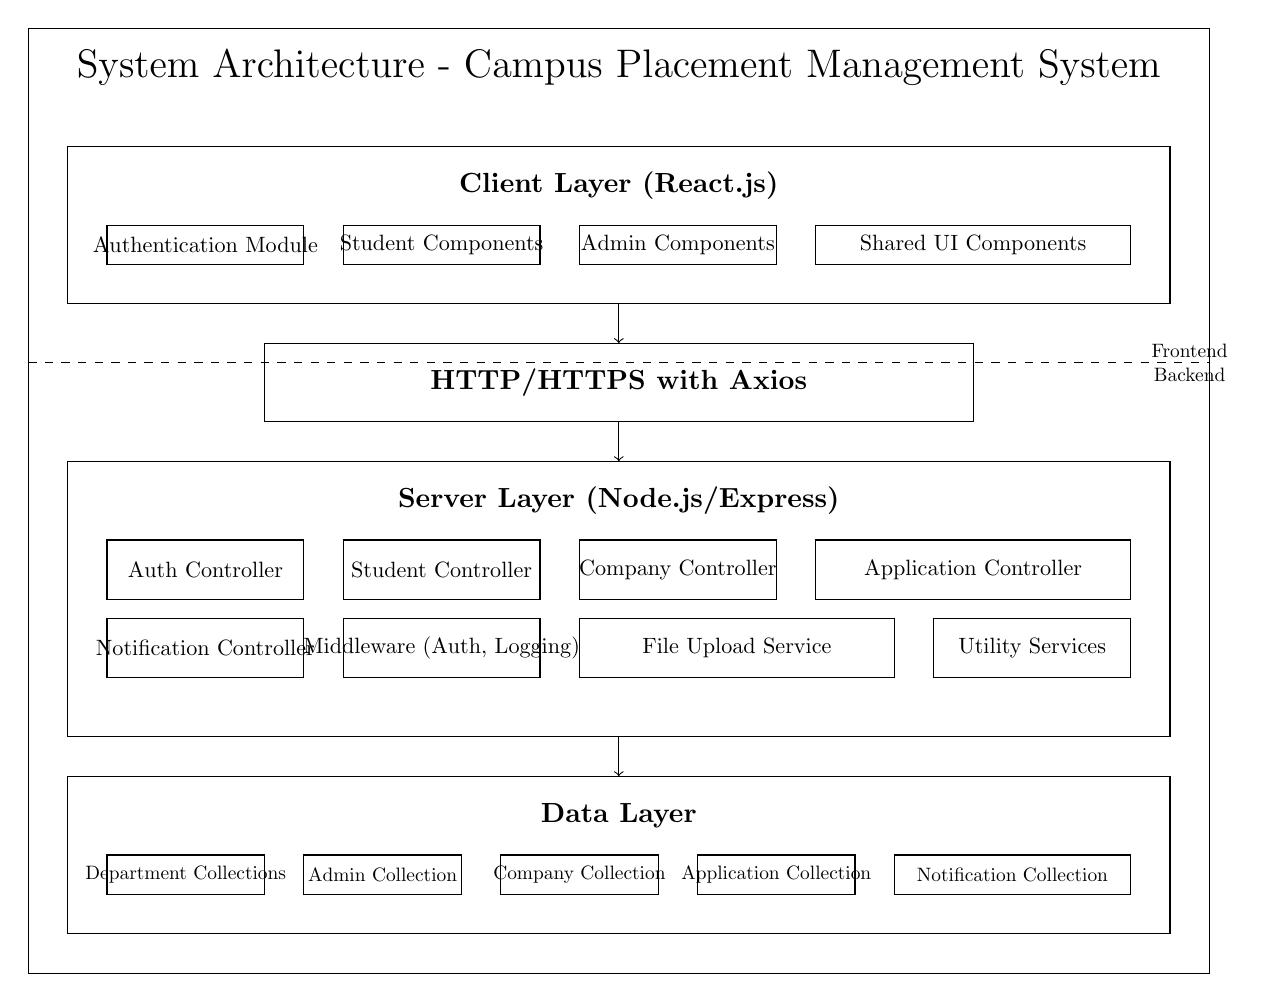
\begin{tikzpicture}
        % Overall box
        \draw (0,0) rectangle (15,12);
        \draw (7.5,11.5) node[align=center] {\Large System Architecture - Campus Placement Management System};
        
        % Client layer
        \draw (0.5,10.5) rectangle (14.5,8.5);
        \draw (7.5,10) node {\textbf{Client Layer (React.js)}};
        
        % Client components
        \draw (1,9.5) rectangle (3.5,9);
        \draw (2.25,9.25) node[scale=0.8] {Authentication Module};
        
        \draw (4,9.5) rectangle (6.5,9);
        \draw (5.25,9.25) node[scale=0.8] {Student Components};
        
        \draw (7,9.5) rectangle (9.5,9);
        \draw (8.25,9.25) node[scale=0.8] {Admin Components};
        
        \draw (10,9.5) rectangle (14,9);
        \draw (12,9.25) node[scale=0.8] {Shared UI Components};
        
        % API Gateway layer
        \draw (3,8) rectangle (12,7);
        \draw (7.5,7.5) node[align=center] {\textbf{HTTP/HTTPS with Axios}};
        
        % Server layer
        \draw (0.5,6.5) rectangle (14.5,3);
        \draw (7.5,6) node[align=center] {\textbf{Server Layer (Node.js/Express)}};
        
        % Server components
        \draw (1,5.5) rectangle (3.5,4.75);
        \draw (2.25,5.125) node[scale=0.8] {Auth Controller};
        
        \draw (4,5.5) rectangle (6.5,4.75);
        \draw (5.25,5.125) node[scale=0.8] {Student Controller};
        
        \draw (7,5.5) rectangle (9.5,4.75);
        \draw (8.25,5.125) node[scale=0.8] {Company Controller};
        
        \draw (10,5.5) rectangle (14,4.75);
        \draw (12,5.125) node[scale=0.8] {Application Controller};
        
        \draw (1,4.5) rectangle (3.5,3.75);
        \draw (2.25,4.125) node[scale=0.8] {Notification Controller};
        
        \draw (4,4.5) rectangle (6.5,3.75);
        \draw (5.25,4.125) node[scale=0.8] {Middleware (Auth, Logging)};
        
        \draw (7,4.5) rectangle (11,3.75);
        \draw (9,4.125) node[scale=0.8] {File Upload Service};
        
        \draw (11.5,4.5) rectangle (14,3.75);
        \draw (12.75,4.125) node[scale=0.8] {Utility Services};
        
        % Database layer
        \draw (0.5,2.5) rectangle (14.5,0.5);
        \draw (7.5,2) node[align=center] {\textbf{Data Layer}};
        
        % Database collections
        \draw (1,1.5) rectangle (3,1);
        \draw (2,1.25) node[scale=0.7] {Department Collections};
        
        \draw (3.5,1.5) rectangle (5.5,1);
        \draw (4.5,1.25) node[scale=0.7] {Admin Collection};
        
        \draw (6,1.5) rectangle (8,1);
        \draw (7,1.25) node[scale=0.7] {Company Collection};
        
        \draw (8.5,1.5) rectangle (10.5,1);
        \draw (9.5,1.25) node[scale=0.7] {Application Collection};
        
        \draw (11,1.5) rectangle (14,1);
        \draw (12.5,1.25) node[scale=0.7] {Notification Collection};
        
        % Connections
        \draw[->] (7.5,8.5) -- (7.5,8);
        \draw[->] (7.5,7) -- (7.5,6.5);
        \draw[->] (7.5,3) -- (7.5,2.5);
        
        % Frontend - Backend division line
        \draw[dashed] (0,7.75) -- (15,7.75);
        \draw (14.75,7.9) node[scale=0.7] {Frontend};
        \draw (14.75,7.6) node[scale=0.7] {Backend};
    \end{tikzpicture}
    \caption{High-level System Architecture}
    \label{fig:system-architecture}
\end{figure}

\section{Security Architecture}
The security architecture implements a defense-in-depth approach with multiple protective layers:

\begin{figure}[H]
    \centering
    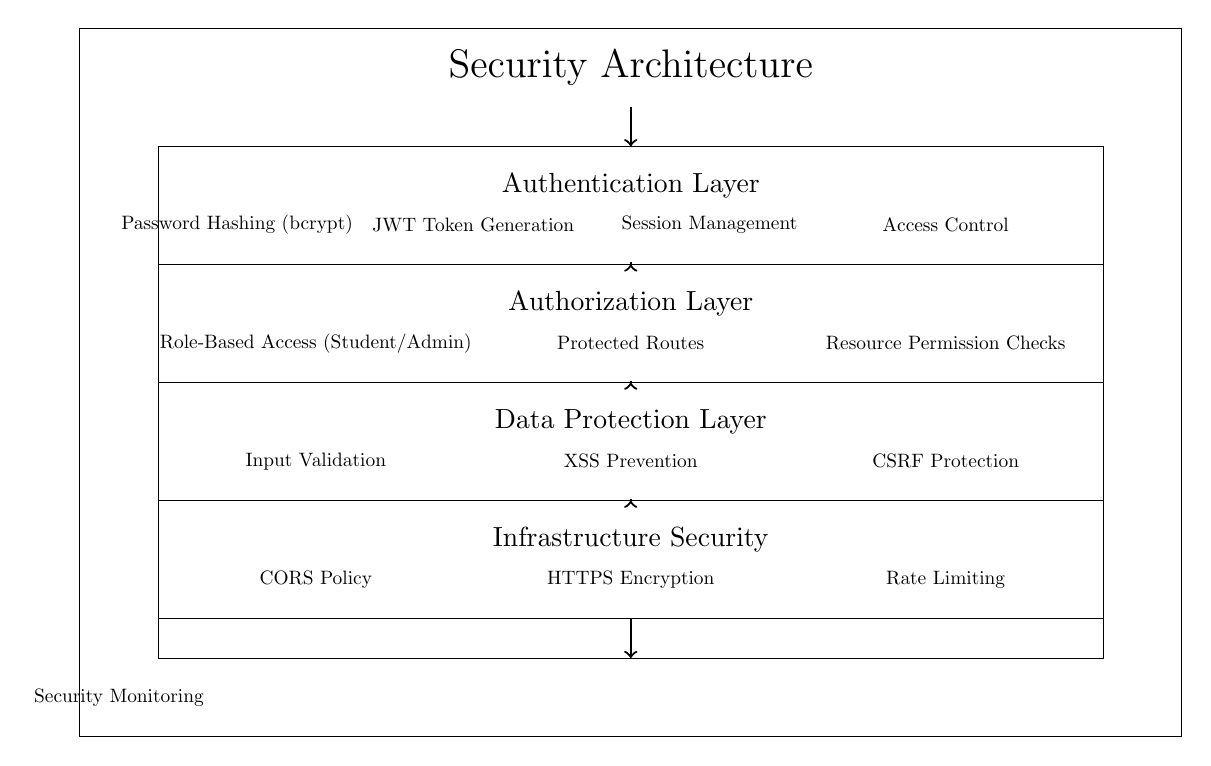
\begin{tikzpicture}
        % Security architecture diagram
        \draw (0,0) rectangle (14,9);
        \draw (7,8.5) node[align=center] {\Large Security Architecture};
        
        % Security layers
        \draw (1,1) rectangle (13,7.5);
        
        % Authentication layer
        \draw (1,7.5) rectangle (13,6);
        \draw (7,7) node {Authentication Layer};
        \draw (2,6.5) node[scale=0.7] {Password Hashing (bcrypt)};
        \draw (5,6.5) node[scale=0.7] {JWT Token Generation};
        \draw (8,6.5) node[scale=0.7] {Session Management};
        \draw (11,6.5) node[scale=0.7] {Access Control};
        
        % Authorization layer
        \draw (1,6) rectangle (13,4.5);
        \draw (7,5.5) node {Authorization Layer};
        \draw (3,5) node[scale=0.7] {Role-Based Access (Student/Admin)};
        \draw (7,5) node[scale=0.7] {Protected Routes};
        \draw (11,5) node[scale=0.7] {Resource Permission Checks};
        
        % Data protection layer
        \draw (1,4.5) rectangle (13,3);
        \draw (7,4) node {Data Protection Layer};
        \draw (3,3.5) node[scale=0.7] {Input Validation};
        \draw (7,3.5) node[scale=0.7] {XSS Prevention};
        \draw (11,3.5) node[scale=0.7] {CSRF Protection};
        
        % Infrastructure security layer
        \draw (1,3) rectangle (13,1.5);
        \draw (7,2.5) node {Infrastructure Security};
        \draw (3,2) node[scale=0.7] {CORS Policy};
        \draw (7,2) node[scale=0.7] {HTTPS Encryption};
        \draw (11,2) node[scale=0.7] {Rate Limiting};
        
        % Monitoring
        \draw (0.5,0.5) node[scale=0.7] {Security Monitoring};
        
        % Arrows showing data flow
        \draw[->, thick] (7,8) -- (7,7.5);
        \draw[->, thick] (7,6) -- (7,6);
        \draw[->, thick] (7,4.5) -- (7,4.5);
        \draw[->, thick] (7,3) -- (7,3);
        \draw[->, thick] (7,1.5) -- (7,1);
    \end{tikzpicture}
    \caption{Security Architecture Overview}
    \label{fig:security-architecture}
\end{figure}

\chapter{Database Design}

\section{Entity-Relationship Diagram}
Figure \ref{fig:erd} shows the entity-relationship diagram for the system, illustrating the relationships between different data entities.

\begin{figure}[H]
    \centering
    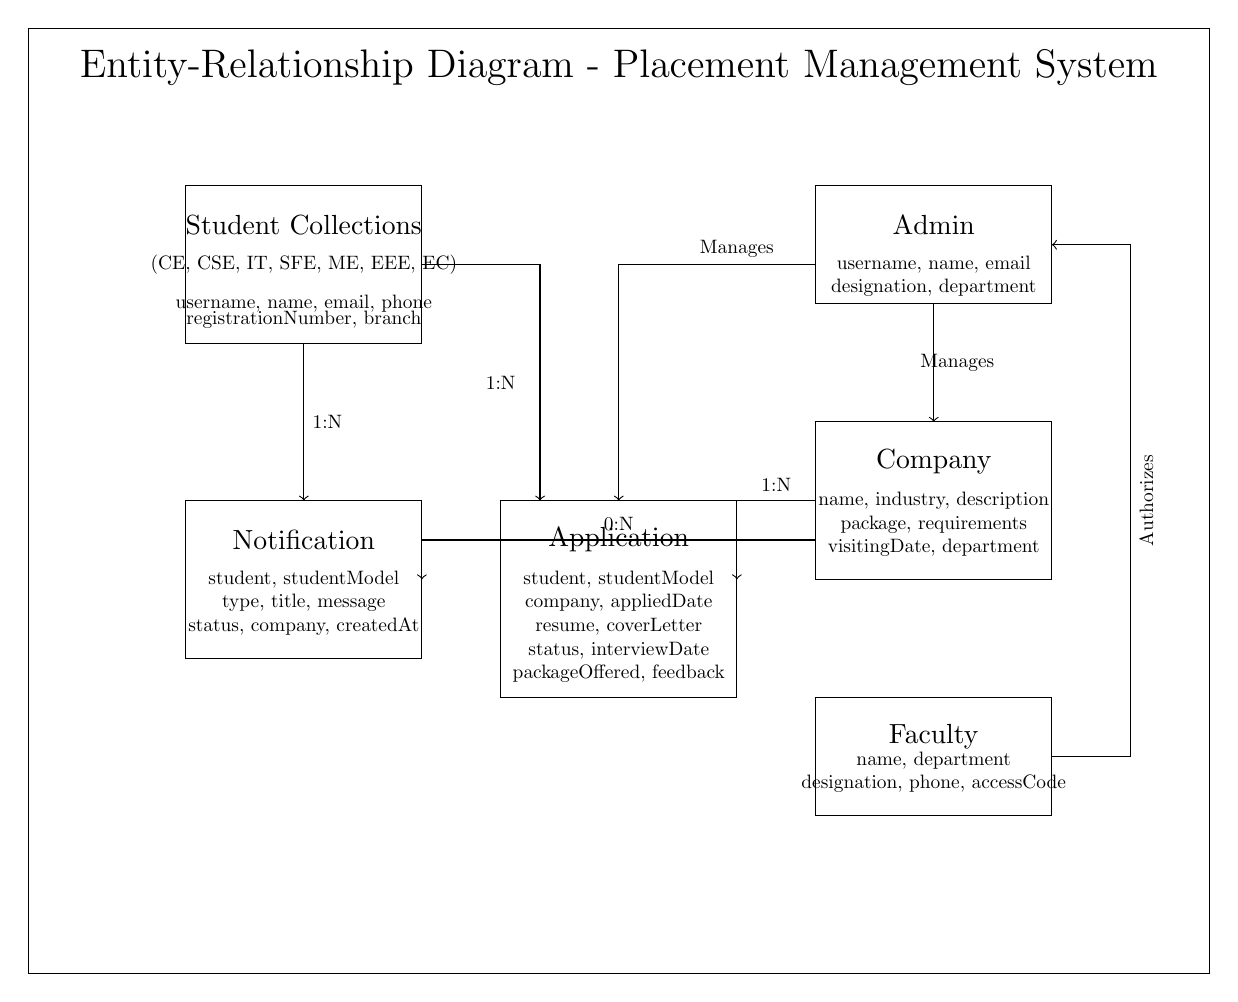
\begin{tikzpicture}
        % ERD container
        \draw (0,0) rectangle (15,12);
        \draw (7.5,11.5) node[align=center] {\Large Entity-Relationship Diagram - Placement Management System};
        
        % Department Student Collections (CE, CSE, etc.)
        \draw (2,10) rectangle (5,8);
        \draw (3.5,9.5) node {Student Collections};
        \draw (3.5,9.0) node[scale=0.7] {(CE, CSE, IT, SFE, ME, EEE, EC)};
        \draw (3.5,8.5) node[scale=0.7] {username, name, email, phone};
        \draw (3.5,8.3) node[scale=0.7] {registrationNumber, branch};
        
        % Admin Entity
        \draw (10,10) rectangle (13,8.5);
        \draw (11.5,9.5) node {Admin};
        \draw (11.5,9.0) node[scale=0.7] {username, name, email};
        \draw (11.5,8.7) node[scale=0.7] {designation, department};
        
        % Company Entity
        \draw (10,7) rectangle (13,5);
        \draw (11.5,6.5) node {Company};
        \draw (11.5,6.0) node[scale=0.7] {name, industry, description};
        \draw (11.5,5.7) node[scale=0.7] {package, requirements};
        \draw (11.5,5.4) node[scale=0.7] {visitingDate, department};
        
        % Application Entity
        \draw (6,6) rectangle (9,3.5);
        \draw (7.5,5.5) node {Application};
        \draw (7.5,5.0) node[scale=0.7] {student, studentModel};
        \draw (7.5,4.7) node[scale=0.7] {company, appliedDate};
        \draw (7.5,4.4) node[scale=0.7] {resume, coverLetter};
        \draw (7.5,4.1) node[scale=0.7] {status, interviewDate};
        \draw (7.5,3.8) node[scale=0.7] {packageOffered, feedback};
        
        % Notification Entity
        \draw (2,6) rectangle (5,4);
        \draw (3.5,5.5) node {Notification};
        \draw (3.5,5.0) node[scale=0.7] {student, studentModel};
        \draw (3.5,4.7) node[scale=0.7] {type, title, message};
        \draw (3.5,4.4) node[scale=0.7] {status, company, createdAt};
        
        % Faculty Entity
        \draw (10,3.5) rectangle (13,2);
        \draw (11.5,3.0) node {Faculty};
        \draw (11.5,2.7) node[scale=0.7] {name, department};
        \draw (11.5,2.4) node[scale=0.7] {designation, phone, accessCode};
        
        % Relationships
        % Student to Application
        \draw[->] (5,9) -- (6.5,9) -- (6.5,6);
        \draw (6,7.5) node[scale=0.7, align=center] {1:N};
        
        % Student to Notification
        \draw[->] (3.5,8) -- (3.5,6);
        \draw (3.8,7) node[scale=0.7, align=center] {1:N};
        
        % Company to Application
        \draw[->] (10,6) -- (9,6) -- (9,5);
        \draw (9.5,6.2) node[scale=0.7, align=center] {1:N};
        
        % Company to Notification (optional)
        \draw[->] (10,5.5) -- (5,5.5) -- (5,5);
        \draw (7.5,5.7) node[scale=0.7, align=center] {0:N};
        
        % Admin manages Company
        \draw[->] (11.5,8.5) -- (11.5,7);
        \draw (11.8,7.75) node[scale=0.7, align=center] {Manages};
        
        % Faculty to Admin
        \draw[->] (13,2.75) -- (14,2.75) -- (14,9.25) -- (13,9.25);
        \draw (14.2,6) node[scale=0.7, align=center, rotate=90] {Authorizes};
        
        % Admin to Applications
        \draw[->] (10,9) -- (7.5,9) -- (7.5,6);
        \draw (9,9.2) node[scale=0.7, align=center] {Manages};
    \end{tikzpicture}
    \caption{Entity-Relationship Diagram}
    \label{fig:erd}
\end{figure}

\chapter{Workflow Diagrams}

\section{User Authentication Workflow}
The authentication workflow implements secure user verification and session management:

\begin{figure}[H]
    \centering
    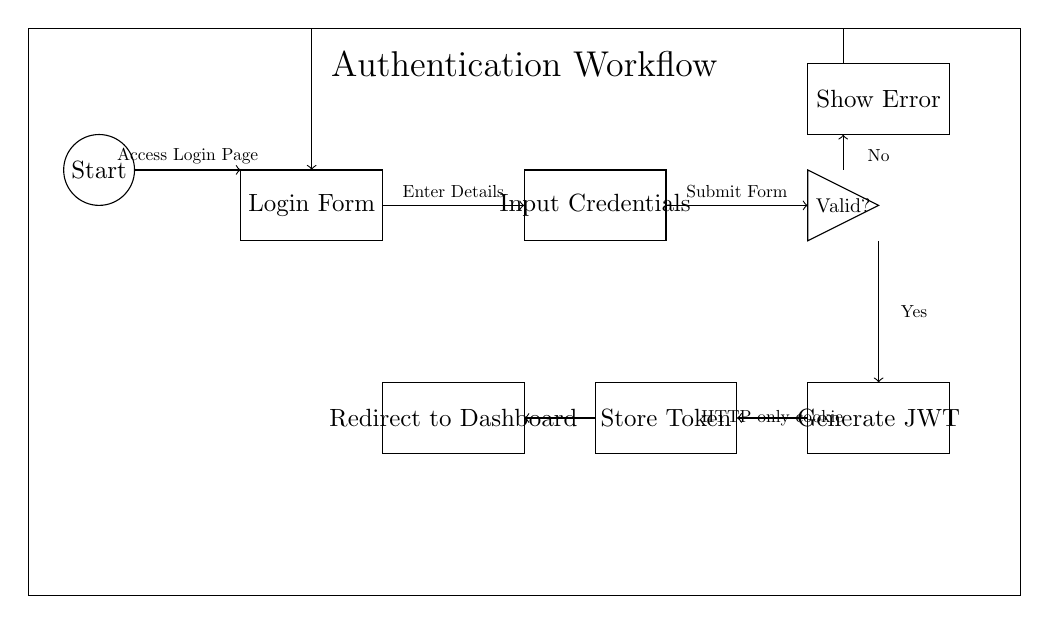
\begin{tikzpicture}[node distance=2cm, scale=0.9, transform shape]
        % Authentication workflow
        \draw (0,0) rectangle (14,8);
        \draw (7,7.5) node[align=center] {\Large Authentication Workflow};
        
        % Start
        \draw (1,6) circle (0.5);
        \draw (1,6) node {Start};
        
        % Login Form
        \draw (3,6) rectangle (5,5);
        \draw (4,5.5) node {Login Form};
        
        % Input Credentials
        \draw (7,6) rectangle (9,5);
        \draw (8,5.5) node {Input Credentials};
        
        % Validation
        \draw (11,6) -- (11,5) -- (12,5.5) -- cycle;
        \draw (11.5,5.5) node[scale=0.8] {Valid?};
        
        % Generate Token
        \draw (11,3) rectangle (13,2);
        \draw (12,2.5) node {Generate JWT};
        
        % Store Token
        \draw (8,3) rectangle (10,2);
        \draw (9,2.5) node {Store Token};
        
        % Redirect
        \draw (5,3) rectangle (7,2);
        \draw (6,2.5) node {Redirect to Dashboard};
        
        % Error
        \draw (11,7.5) rectangle (13,6.5);
        \draw (12,7) node {Show Error};
        
        % Connections
        \draw[->] (1.5,6) -- (3,6);
        \draw[->] (5,5.5) -- (7,5.5);
        \draw[->] (9,5.5) -- (11,5.5);
        \draw[->] (12,5) -- (12,3);
        \draw[->] (11,2.5) -- (10,2.5);
        \draw[->] (8,2.5) -- (7,2.5);
        \draw[->] (11.5,6) -- (11.5,6.5);
        \draw[->] (11.5,7.5) -- (11.5,8) -- (4,8) -- (4,6);
        
        % Labels
        \draw (2.25,6.2) node[scale=0.7] {Access Login Page};
        \draw (6,5.7) node[scale=0.7] {Enter Details};
        \draw (10,5.7) node[scale=0.7] {Submit Form};
        \draw (12.5,4) node[scale=0.7] {Yes};
        \draw (12,6.2) node[scale=0.7] {No};
        \draw (10.5,2.5) node[scale=0.7] {HTTP-only cookie};
    \end{tikzpicture}
    \caption{User Authentication Workflow}
    \label{fig:auth-workflow}
\end{figure}

The authentication workflow includes:
\begin{itemize}
    \item Frontend validation of credentials using React Hook Form
    \item Backend validation against the appropriate student or admin collection
    \item Secure password checking using bcrypt's compare function
    \item JWT token generation with user role and department encoded
    \item HTTP-only cookie storage to prevent XSS attacks
    \item Session timeout after 30 minutes of inactivity
\end{itemize}

\section{Application Submission Workflow}
The application submission process ensures proper validation and tracking:

\begin{figure}[H]
    \centering
    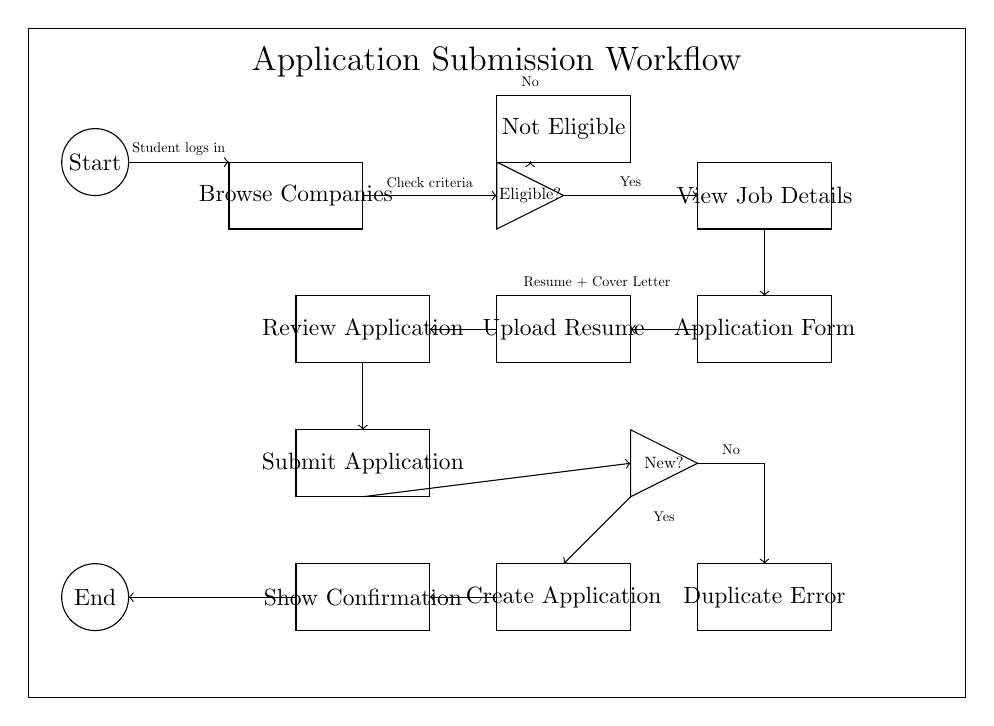
\begin{tikzpicture}[node distance=2cm, scale=0.85, transform shape]
        % Application workflow
        \draw (0,0) rectangle (14,10);
        \draw (7,9.5) node[align=center] {\Large Application Submission Workflow};
        
        % Start
        \draw (1,8) circle (0.5);
        \draw (1,8) node {Start};
        
        % Browse Companies
        \draw (3,8) rectangle (5,7);
        \draw (4,7.5) node {Browse Companies};
        
        % Eligibility Check
        \draw (7,8) -- (7,7) -- (8,7.5) -- cycle;
        \draw (7.5,7.5) node[scale=0.7] {Eligible?};
        
        % View Job Details
        \draw (10,8) rectangle (12,7);
        \draw (11,7.5) node {View Job Details};
        
        % Not Eligible Message
        \draw (7,9) rectangle (9,8);
        \draw (8,8.5) node {Not Eligible};
        
        % Application Form
        \draw (10,6) rectangle (12,5);
        \draw (11,5.5) node {Application Form};
        
        % Upload Resume
        \draw (7,6) rectangle (9,5);
        \draw (8,5.5) node {Upload Resume};
        
        % Review Application
        \draw (4,6) rectangle (6,5);
        \draw (5,5.5) node {Review Application};
        
        % Submit Application
        \draw (4,4) rectangle (6,3);
        \draw (5,3.5) node {Submit Application};
        
        % Duplicate Check
        \draw (9,4) -- (9,3) -- (10,3.5) -- cycle;
        \draw (9.5,3.5) node[scale=0.7] {New?};
        
        % Duplicate Error
        \draw (10,2) rectangle (12,1);
        \draw (11,1.5) node {Duplicate Error};
        
        % Create Application
        \draw (7,2) rectangle (9,1);
        \draw (8,1.5) node {Create Application};
        
        % Confirmation
        \draw (4,2) rectangle (6,1);
        \draw (5,1.5) node {Show Confirmation};
        
        % End
        \draw (1,1.5) circle (0.5);
        \draw (1,1.5) node {End};
        
        % Connections
        \draw[->] (1.5,8) -- (3,8);
        \draw[->] (5,7.5) -- (7,7.5);
        \draw[->] (8,7.5) -- (10,7.5);
        \draw[->] (7.5,8) -- (7.5,8);
        \draw[->] (11,7) -- (11,6);
        \draw[->] (10,5.5) -- (9,5.5);
        \draw[->] (7,5.5) -- (6,5.5);
        \draw[->] (5,5) -- (5,4);
        \draw[->] (5,3) -- (9,3.5);
        \draw[->] (10,3.5) -- (11,3.5) -- (11,2);
        \draw[->] (9,3) -- (8,2);
        \draw[->] (7,1.5) -- (6,1.5);
        \draw[->] (4,1.5) -- (1.5,1.5);
        
        % Labels with reduced scale
        \draw (2.25,8.2) node[scale=0.6] {Student logs in};
        \draw (6,7.7) node[scale=0.6] {Check criteria};
        \draw (9,7.7) node[scale=0.6] {Yes};
        \draw (7.5,9.2) node[scale=0.6] {No};
        \draw (8.5,6.2) node[scale=0.6] {Resume + Cover Letter};
        \draw (10.5,3.7) node[scale=0.6] {No};
        \draw (9.5,2.7) node[scale=0.6] {Yes};
    \end{tikzpicture}
    \caption{Application Submission Workflow}
    \label{fig:application-workflow}
\end{figure}

The application submission process implements several key validations:
\begin{itemize}
    \item Automatic eligibility filtering based on student's department and CGPA
    \item File type validation for resume uploads (PDF only)
    \item File size limits (5MB maximum)
    \item Duplicate application prevention through database queries
    \item Custom validation rules for cover letters and additional information
    \item Status tracking with timestamps for each stage transition
\end{itemize}

\section{Notification Delivery Workflow}
The notification system ensures timely delivery of important updates:

\begin{figure}[H]
    \centering
    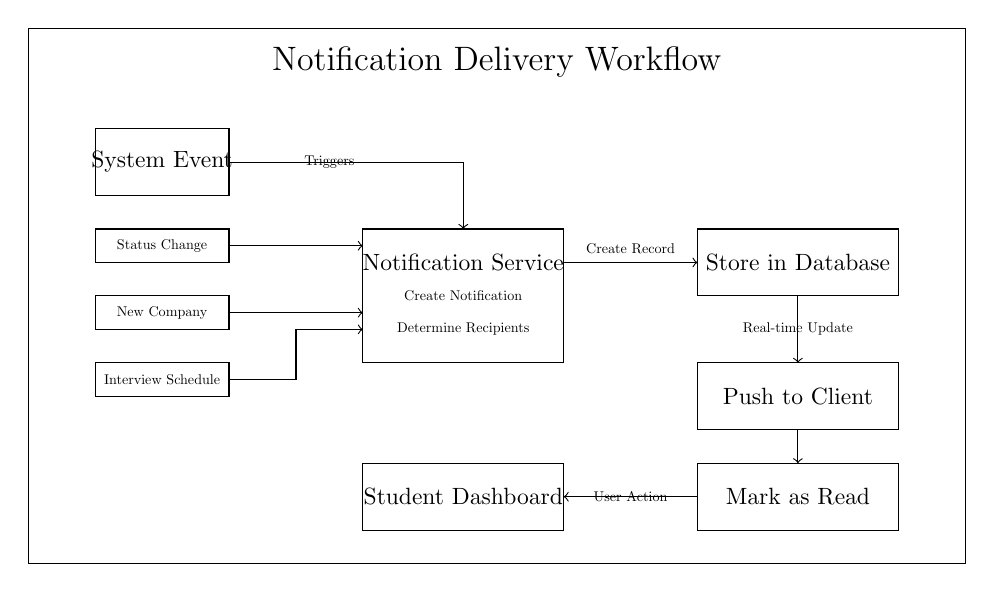
\begin{tikzpicture}[node distance=2cm, scale=0.85, transform shape]
        % Notification workflow
        \draw (0,0) rectangle (14,8);
        \draw (7,7.5) node[align=center] {\Large Notification Delivery Workflow};
        
        % Trigger Events
        \draw (1,6.5) rectangle (3,5.5);
        \draw (2,6) node {System Event};
        
        % Event Types
        \draw (1,5) rectangle (3,4.5);
        \draw (2,4.75) node[scale=0.6] {Status Change};
        
        \draw (1,4) rectangle (3,3.5);
        \draw (2,3.75) node[scale=0.6] {New Company};
        
        \draw (1,3) rectangle (3,2.5);
        \draw (2,2.75) node[scale=0.6] {Interview Schedule};
        
        % Process Notification
        \draw (5,5) rectangle (8,3);
        \draw (6.5,4.5) node {Notification Service};
        \draw (6.5,4) node[scale=0.6] {Create Notification};
        \draw (6.5,3.5) node[scale=0.6] {Determine Recipients};
        
        % Store Notification
        \draw (10,5) rectangle (13,4);
        \draw (11.5,4.5) node {Store in Database};
        
        % Delivery Methods
        \draw (10,3) rectangle (13,2);
        \draw (11.5,2.5) node {Push to Client};
        
        % Student Views
        \draw (5,1.5) rectangle (8,0.5);
        \draw (6.5,1) node {Student Dashboard};
        
        % User Interactions
        \draw (10,1.5) rectangle (13,0.5);
        \draw (11.5,1) node {Mark as Read};
        
        % Connections
        \draw[->] (3,6) -- (6.5,6) -- (6.5,5);
        \draw[->] (3,4.75) -- (5,4.75);
        \draw[->] (3,3.75) -- (5,3.75);
        \draw[->] (3,2.75) -- (4,2.75) -- (4,3.5) -- (5,3.5);
        \draw[->] (8,4.5) -- (10,4.5);
        \draw[->] (11.5,4) -- (11.5,3);
        \draw[->] (11.5,2) -- (11.5,1.5);
        \draw[->] (10,1) -- (8,1);
        
        % Labels
        \draw (4.5,6) node[scale=0.6] {Triggers};
        \draw (9,4.7) node[scale=0.6] {Create Record};
        \draw (11.5,3.5) node[scale=0.6] {Real-time Update};
        \draw (9,1) node[scale=0.6] {User Action};
    \end{tikzpicture}
    \caption{Notification Delivery Workflow}
    \label{fig:notification-workflow}
\end{figure}

The notification system implements several types of notifications:
\begin{itemize}
    \item Application status updates (Applied, Under Review, Interview Scheduled, etc.)
    \item New company arrivals matching student's department
    \item Interview schedule confirmations and reminders
    \item Administrative announcements and placement information
    \item System-wide notifications for maintenance or important deadlines
\end{itemize}

\chapter{Project File Structure}

\section{Frontend Structure}
The React frontend follows a well-organized component-based architecture:

\begin{figure}[H]
    \centering
    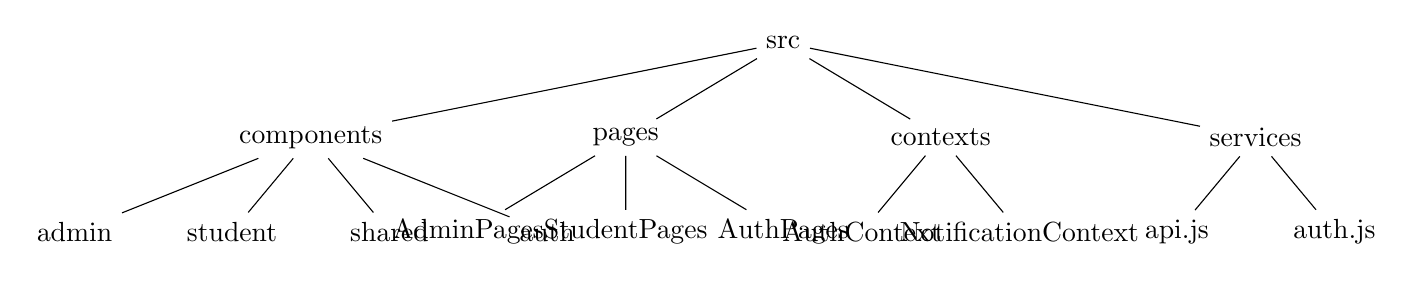
\begin{tikzpicture}[level distance=1.2cm, sibling distance=3cm, 
                        level 1/.style={sibling distance=4cm},
                        level 2/.style={sibling distance=2cm}]
        \node {src}
            child {node {components}
                child {node {admin}}
                child {node {student}}
                child {node {shared}}
                child {node {auth}}
            }
            child {node {pages}
                child {node {AdminPages}}
                child {node {StudentPages}}
                child {node {AuthPages}}
            }
            child {node {contexts}
                child {node {AuthContext}}
                child {node {NotificationContext}}
            }
            child {node {services}
                child {node {api.js}}
                child {node {auth.js}}
            };
    \end{tikzpicture}
    \caption{Frontend Project Structure}
    \label{fig:frontend-structure}
\end{figure}

The React application follows best practices for organization:
\begin{itemize}
    \item \textbf{Components:} Reusable UI elements organized by user type and functionality
    \item \textbf{Pages:} Complete page layouts combining multiple components
    \item \textbf{Contexts:} React Context API implementations for global state management
    \item \textbf{Services:} Modules for external API communication and business logic
    \item \textbf{Utils:} Helper functions and utilities for common operations
    \item \textbf{Hooks:} Custom React hooks for reusable stateful logic
    \item \textbf{Assets:} Static resources including images, icons, and stylesheets
\end{itemize}

\section{Backend Structure}
The Node.js/Express backend is organized following the MVC pattern:

\begin{figure}[H]
    \centering
    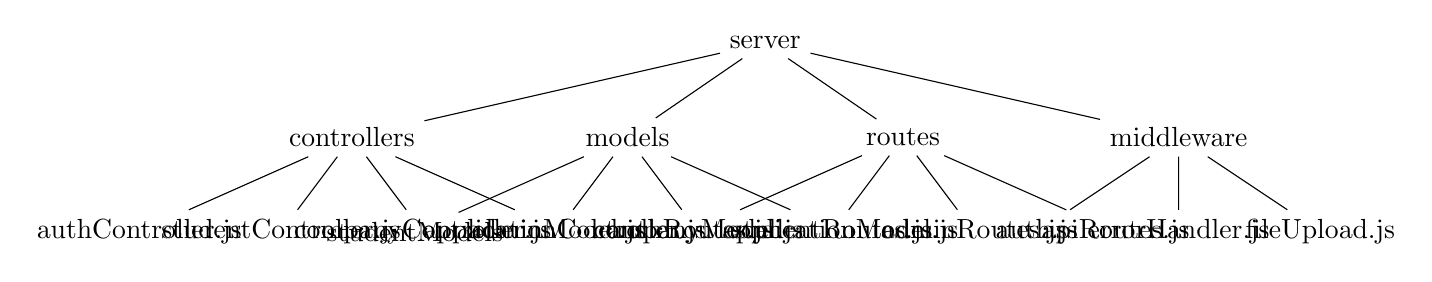
\begin{tikzpicture}[level distance=1.2cm, sibling distance=3cm,
                        level 1/.style={sibling distance=3.5cm},
                        level 2/.style={sibling distance=1.8cm}]
        \node {server}
            child {node {controllers}
                child {node {authController.js}}
                child {node {studentController.js}}
                child {node {companyController.js}}
                child {node {applicationController.js}}
            }
            child {node {models}
                child {node {studentModels}}
                child {node {adminModel.js}}
                child {node {companyModel.js}}
                child {node {applicationModel.js}}
            }
            child {node {routes}
                child {node {authRoutes.js}}
                child {node {studentRoutes.js}}
                child {node {adminRoutes.js}}
                child {node {apiRoutes.js}}
            }
            child {node {middleware}
                child {node {auth.js}}
                child {node {errorHandler.js}}
                child {node {fileUpload.js}}
            };
    \end{tikzpicture}
    \caption{Backend Project Structure}
    \label{fig:backend-structure}
\end{figure}

The backend organization incorporates:
\begin{itemize}
    \item \textbf{Controllers:} Handle request processing and business logic
    \item \textbf{Models:} MongoDB schemas and data access methods
    \item \textbf{Routes:} API endpoint definitions and routing logic
    \item \textbf{Middleware:} Request processing functions for authentication, validation, etc.
    \item \textbf{Config:} Configuration settings for development and production environments
    \item \textbf{Utils:} Helper functions for common operations
    \item \textbf{Uploads:} Storage for user-uploaded files (resumes, etc.)
\end{itemize}

\chapter{Implementation Details}

\section{Authentication Implementation}
The authentication system leverages Passport.js with custom strategies:

\begin{figure}[H]
    \centering
    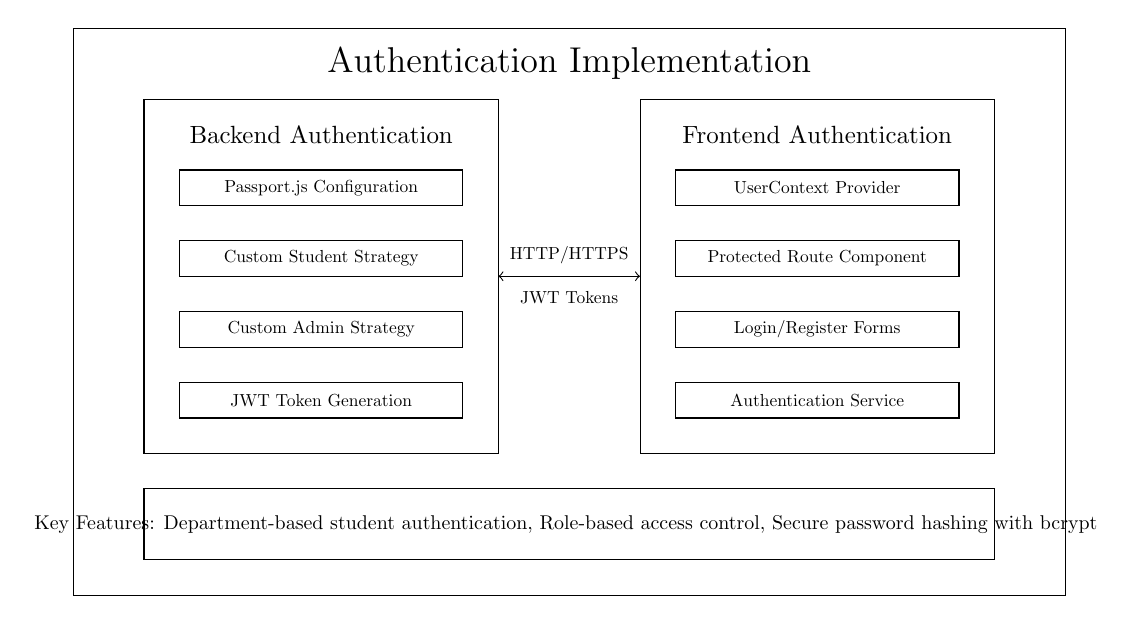
\begin{tikzpicture}[node distance=2cm, scale=0.9, transform shape]
        % Code structure diagram
        \draw (0,0) rectangle (14,8);
        \draw (7,7.5) node[align=center] {\Large Authentication Implementation};
        
        % Backend Authentication
        \draw (1,7) rectangle (6,2);
        \draw (3.5,6.5) node {Backend Authentication};
        
        \draw (1.5,6) rectangle (5.5,5.5);
        \draw (3.5,5.75) node[scale=0.7] {Passport.js Configuration};
        
        \draw (1.5,5) rectangle (5.5,4.5);
        \draw (3.5,4.75) node[scale=0.7] {Custom Student Strategy};
        
        \draw (1.5,4) rectangle (5.5,3.5);
        \draw (3.5,3.75) node[scale=0.7] {Custom Admin Strategy};
        
        \draw (1.5,3) rectangle (5.5,2.5);
        \draw (3.5,2.75) node[scale=0.7] {JWT Token Generation};
        
        % Frontend Authentication
        \draw (8,7) rectangle (13,2);
        \draw (10.5,6.5) node {Frontend Authentication};
        
        \draw (8.5,6) rectangle (12.5,5.5);
        \draw (10.5,5.75) node[scale=0.7] {UserContext Provider};
        
        \draw (8.5,5) rectangle (12.5,4.5);
        \draw (10.5,4.75) node[scale=0.7] {Protected Route Component};
        
        \draw (8.5,4) rectangle (12.5,3.5);
        \draw (10.5,3.75) node[scale=0.7] {Login/Register Forms};
        
        \draw (8.5,3) rectangle (12.5,2.5);
        \draw (10.5,2.75) node[scale=0.7] {Authentication Service};
        
        % Connection
        \draw[<->] (6,4.5) -- (8,4.5);
        \draw (7,4.8) node[scale=0.7] {HTTP/HTTPS};
        \draw (7,4.2) node[scale=0.7] {JWT Tokens};
        
        % Key functionality
        \draw (1,1.5) rectangle (13,0.5);
        \draw (7,1) node[align=center, scale=0.8] {
            Key Features: Department-based student authentication, 
            Role-based access control, Secure password hashing with bcrypt
        };
    \end{tikzpicture}
    \caption{Authentication Implementation Architecture}
    \label{fig:auth-implementation}
\end{figure}

\subsection{Authentication Code Samples}

\subsubsection{Backend JWT Authentication}
The backend implements custom JWT-based authentication:

\begin{lstlisting}[language=JavaScript, caption=JWT Authentication Middleware]
// Middleware to verify JWT tokens
const auth = (req, res, next) => {
  try {
    const token = req.cookies.token;
    
    if (!token) {
      return res.status(401).json({ message: 'No authentication token, access denied' });
    }
    
    const verified = jwt.verify(token, process.env.JWT_SECRET);
    req.user = verified;
    
    // Attach model name based on user role for database operations
    if (req.user.role === 'student') {
      req.model = req.user.department; // CE, CSE, IT, etc.
    }
    
    next();
  } catch (err) {
    res.status(401).json({ message: 'Token verification failed' });
  }
};

// Role-based authorization middleware
const authorize = (roles = []) => {
  return (req, res, next) => {
    if (!req.user) {
      return res.status(401).json({ message: 'Authentication required' });
    }
    
    if (roles.length && !roles.includes(req.user.role)) {
      return res.status(403).json({ message: 'Insufficient permissions' });
    }
    
    next();
  };
};
\end{lstlisting}

\subsubsection{React Protected Routes}
The frontend implements protected routes using React Router:

\begin{lstlisting}[language=JavaScript, caption=Protected Route Component]
// Component to protect routes based on authentication and role
const ProtectedRoute = ({ component: Component, roles, ...rest }) => {
  const { user, isLoading } = useAuth();
  
  return (
    <Route
      {...rest}
      render={(props) => {
        // Show loading spinner while checking authentication
        if (isLoading) {
          return <LoadingSpinner />;
        }
        
        // Redirect to login if not authenticated
        if (!user) {
          return <Redirect to={{
            pathname: '/login',
            state: { from: props.location }
          }} />;
        }
        
        // Check if user has required role
        if (roles && !roles.includes(user.role)) {
          return <Redirect to="/unauthorized" />;
        }
        
        // Render requested component if all checks pass
        return <Component {...props} />;
      }}
    />
  );
};
\end{lstlisting}

\section{Notification System Implementation}
The notification system architecture enables real-time updates:

\begin{figure}[H]
    \centering
    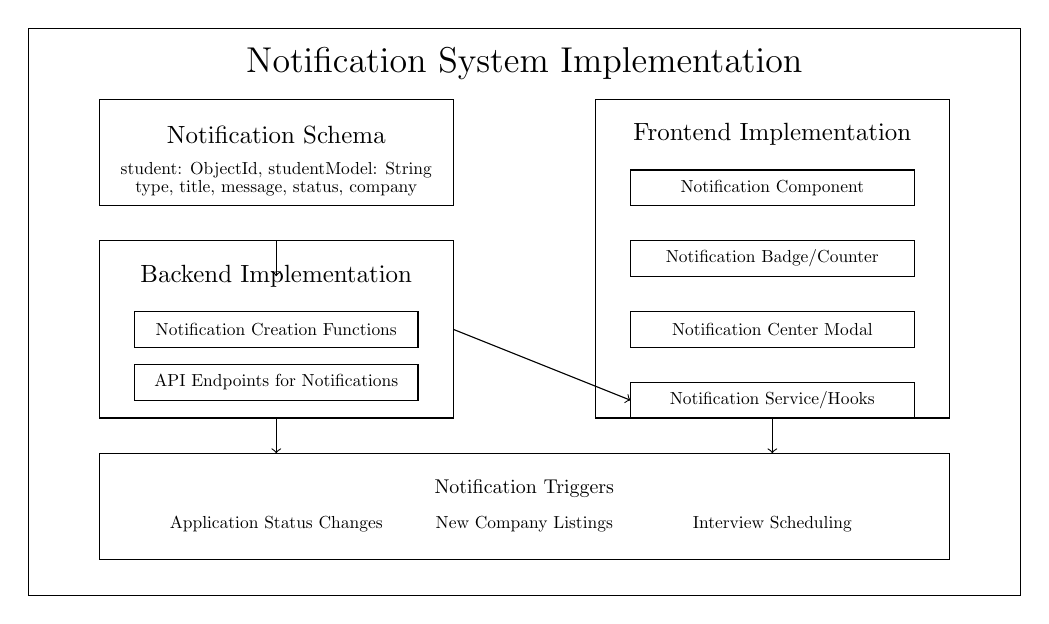
\begin{tikzpicture}[node distance=2cm, scale=0.9, transform shape]
        % Notification system diagram
        \draw (0,0) rectangle (14,8);
        \draw (7,7.5) node[align=center] {\Large Notification System Implementation};
        
        % Database Model
        \draw (1,7) rectangle (6,5.5);
        \draw (3.5,6.5) node {Notification Schema};
        \draw (3.5,6) node[scale=0.7] {student: ObjectId, studentModel: String};
        \draw (3.5,5.75) node[scale=0.7] {type, title, message, status, company};
        
        % Backend Components
        \draw (1,5) rectangle (6,2.5);
        \draw (3.5,4.5) node {Backend Implementation};
        
        \draw (1.5,4) rectangle (5.5,3.5);
        \draw (3.5,3.75) node[scale=0.7] {Notification Creation Functions};
        
        \draw (1.5,3.25) rectangle (5.5,2.75);
        \draw (3.5,3) node[scale=0.7] {API Endpoints for Notifications};
        
        % Frontend Components
        \draw (8,7) rectangle (13,2.5);
        \draw (10.5,6.5) node {Frontend Implementation};
        
        \draw (8.5,6) rectangle (12.5,5.5);
        \draw (10.5,5.75) node[scale=0.7] {Notification Component};
        
        \draw (8.5,5) rectangle (12.5,4.5);
        \draw (10.5,4.75) node[scale=0.7] {Notification Badge/Counter};
        
        \draw (8.5,4) rectangle (12.5,3.5);
        \draw (10.5,3.75) node[scale=0.7] {Notification Center Modal};
        
        \draw (8.5,3) rectangle (12.5,2.5);
        \draw (10.5,2.75) node[scale=0.7] {Notification Service/Hooks};
        
        % Integration points
        \draw (1,2) rectangle (13,0.5);
        \draw (7,1.5) node[scale=0.8] {Notification Triggers};
        \draw (3.5,1) node[scale=0.7] {Application Status Changes};
        \draw (7,1) node[scale=0.7] {New Company Listings};
        \draw (10.5,1) node[scale=0.7] {Interview Scheduling};
        
        % Connections
        \draw[->] (6,3.75) -- (8.5,2.75);
        \draw[->] (3.5,2.5) -- (3.5,2);
        \draw[->] (10.5,2.5) -- (10.5,2);
        \draw[->] (3.5,5) -- (3.5,4.5);
    \end{tikzpicture}
    \caption{Notification System Implementation}
    \label{fig:notification-implementation}
\end{figure}

\subsection{Notification Code Samples}

\subsubsection{Notification Creation}
The backend implements notification creation functionality:

\begin{lstlisting}[language=JavaScript, caption=Notification Creation Function]
// Function to create a new notification
const createNotification = async (studentId, studentModel, options) => {
  try {
    const { type, title, message, company = null } = options;
    
    const notification = new Notification({
      student: studentId,
      studentModel,
      type,
      title,
      message,
      status: 'unread',
      company,
      createdAt: new Date()
    });
    
    await notification.save();
    
    // Emit real-time notification if Socket.IO is used
    if (io) {
      io.to(`student-${studentId}`).emit('notification', {
        id: notification._id,
        type,
        title,
        message
      });
    }
    
    return notification;
  } catch (error) {
    console.error('Notification creation error:', error);
    throw error;
  }
};

// Example: Create notification for application status change
const notifyApplicationStatusChange = async (application, newStatus) => {
  const { student, studentModel, company } = application;
  
  // Get company name
  const companyDoc = await Company.findById(company);
  const companyName = companyDoc ? companyDoc.name : 'a company';
  
  // Create notification based on status
  const notificationOptions = {
    type: 'application',
    company,
    title: `Application Status Updated`,
    message: `Your application for ${companyName} has been updated to "${newStatus}"`
  };
  
  return createNotification(student, studentModel, notificationOptions);
};
\end{lstlisting}

\subsubsection{Frontend Notification Component}
The React notification badge and dropdown component:

\begin{lstlisting}[language=JavaScript, caption=Notification Badge Component]
const NotificationBadge = () => {
  const { notifications, markAsRead } = useNotifications();
  const [isOpen, setIsOpen] = useState(false);
  
  const unreadCount = useMemo(() => {
    return notifications.filter(n => n.status === 'unread').length;
  }, [notifications]);
  
  const toggleNotifications = () => setIsOpen(!isOpen);
  
  const handleMarkAsRead = (id) => {
    markAsRead(id);
  };
  
  return (
    <div className="notification-container">
      <button className="notification-bell" onClick={toggleNotifications}>
        <BellIcon />
        {unreadCount > 0 && (
          <span className="notification-badge">{unreadCount}</span>
        )}
      </button>
      
      {isOpen && (
        <div className="notification-dropdown">
          <div className="notification-header">
            <h3>Notifications</h3>
            {unreadCount > 0 && (
              <button onClick={() => markAsRead('all')}>
                Mark all as read
              </button>
            )}
          </div>
          
          <div className="notification-list">
            {notifications.length === 0 ? (
              <p className="empty-state">No notifications yet</p>
            ) : (
              notifications.slice(0, 5).map(notification => (
                <div 
                  key={notification._id}
                  className={`notification-item ${notification.status === 'unread' ? 'unread' : ''}`}
                  onClick={() => handleMarkAsRead(notification._id)}
                >
                  <div className="notification-icon">
                    {getIconForType(notification.type)}
                  </div>
                  <div className="notification-content">
                    <h4>{notification.title}</h4>
                    <p>{notification.message}</p>
                    <span className="notification-time">
                      {formatTimeAgo(notification.createdAt)}
                    </span>
                  </div>
                </div>
              ))
            )}
          </div>
          
          <div className="notification-footer">
            <Link to="/notifications">View all notifications</Link>
          </div>
        </div>
      )}
    </div>
  );
};
\end{lstlisting}

\section{Application Management Implementation}
The application management system handles the lifecycle of student job applications:

\begin{lstlisting}[language=JavaScript, caption=Application Status Update Function]
// Update application status with appropriate notifications
const updateApplicationStatus = async (req, res) => {
  try {
    const { id } = req.params;
    const { status, feedback, interviewDate, packageOffered } = req.body;
    
    // Find the application
    const application = await Application.findById(id);
    if (!application) {
      return res.status(404).json({ message: 'Application not found' });
    }
    
    // Update application with new information
    application.status = status;
    
    if (feedback) application.feedback = feedback;
    if (interviewDate) application.interviewDate = new Date(interviewDate);
    if (packageOffered) application.packageOffered = packageOffered;
    
    // Save updated application
    await application.save();
    
    // Create notification for the student
    await notifyApplicationStatusChange(application, status);
    
    // Create interview notification if status is "Interview Scheduled"
    if (status === 'Interview Scheduled' && interviewDate) {
      const company = await Company.findById(application.company);
      const companyName = company ? company.name : 'a company';
      
      await createNotification(
        application.student, 
        application.studentModel,
        {
          type: 'interview',
          company: application.company,
          title: 'Interview Scheduled',
          message: `Your interview with ${companyName} is scheduled for ${new Date(interviewDate).toLocaleString()}`,
        }
      );
    }
    
    res.status(200).json({ 
      message: 'Application updated successfully',
      application
    });
  } catch (error) {
    console.error('Error updating application:', error);
    res.status(500).json({ message: 'Server error', error: error.message });
  }
};
\end{lstlisting}

\chapter{User Interface Design}

\section{Key Interface Components}
The system features a responsive, user-friendly interface designed for different user roles:

\begin{figure}[H]
    \centering
    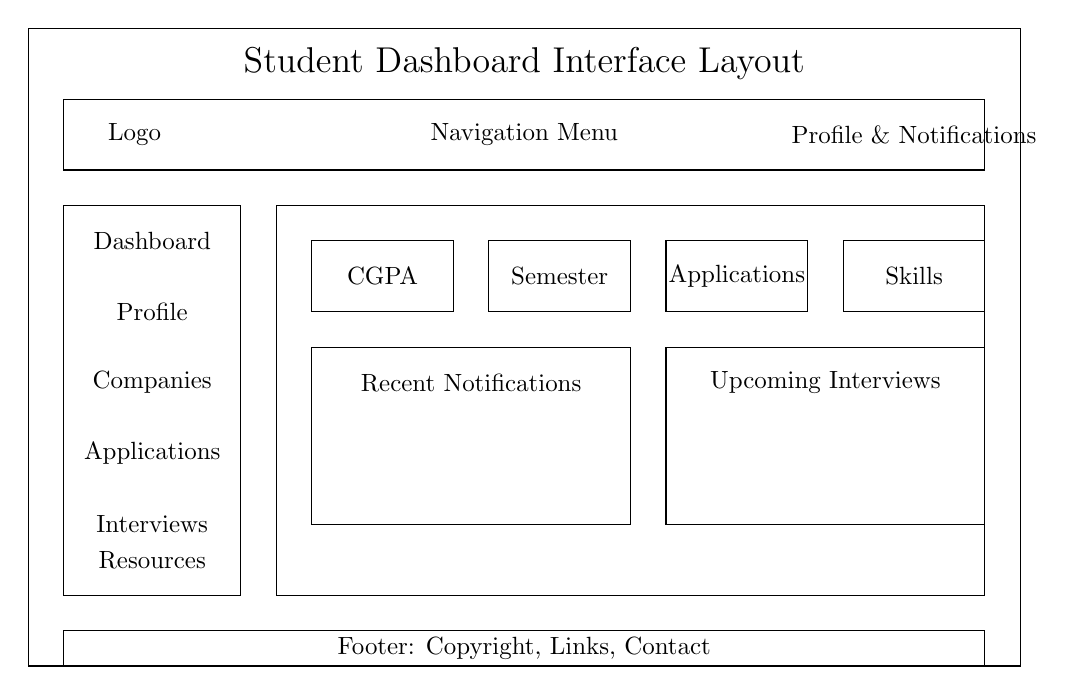
\begin{tikzpicture}[node distance=2cm, scale=0.9, transform shape]
        % UI Layout
        \draw (0,0) rectangle (14,9);
        \draw (7,8.5) node[align=center] {\Large Student Dashboard Interface Layout};
        
        % Header
        \draw (0.5,8) rectangle (13.5,7);
        \draw (1.5,7.5) node[align=left] {Logo};
        \draw (7,7.5) node {Navigation Menu};
        \draw (12.5,7.5) node {Profile \& Notifications};
        
        % Sidebar
        \draw (0.5,6.5) rectangle (3,1);
        \draw (1.75,6) node {Dashboard};
        \draw (1.75,5) node {Profile};
        \draw (1.75,4) node {Companies};
        \draw (1.75,3) node {Applications};
        \draw (1.75,2) node {Interviews};
        \draw (1.75,1.5) node {Resources};
        
        % Main Content
        \draw (3.5,6.5) rectangle (13.5,1);
        
        % Stats Cards
        \draw (4,6) rectangle (6,5);
        \draw (5,5.5) node {CGPA};
        
        \draw (6.5,6) rectangle (8.5,5);
        \draw (7.5,5.5) node {Semester};
        
        \draw (9,6) rectangle (11,5);
        \draw (10,5.5) node {Applications};
        
        \draw (11.5,6) rectangle (13.5,5);
        \draw (12.5,5.5) node {Skills};
        
        % Recent Notifications
        \draw (4,4.5) rectangle (8.5,2);
        \draw (6.25,4) node {Recent Notifications};
        
        % Upcoming Interviews
        \draw (9,4.5) rectangle (13.5,2);
        \draw (11.25,4) node {Upcoming Interviews};
        
        % Footer
        \draw (0.5,0.5) rectangle (13.5,0);
        \draw (7,0.25) node {Footer: Copyright, Links, Contact};
    \end{tikzpicture}
    \caption{Student Dashboard Interface Layout}
    \label{fig:student-dashboard}
\end{figure}

\section{Interface Screenshots}
Below are key screenshots from the Campus Placement Management System:

\subsection{Student Dashboard}
\begin{figure}[H]
    \centering
    \fbox{\parbox{0.8\textwidth}{
        \centering
        [Student Dashboard Screenshot]\\
        This screenshot would show the student dashboard with quick statistics,\\
        recent notifications, and upcoming interviews.
    }}
    \caption{Student Dashboard}
    \label{fig:student-dashboard-screenshot}
\end{figure}

\subsection{Company Listing}
\begin{figure}[H]
    \centering
    \fbox{\parbox{0.8\textwidth}{
        \centering
        [Company Listing Screenshot]\\
        This screenshot would show the available companies with filtering options,\\
        eligibility indicators, and application buttons.
    }}
    \caption{Company Listing Interface}
    \label{fig:company-listing-screenshot}
\end{figure}

\subsection{Application Form}
\begin{figure}[H]
    \centering
    \fbox{\parbox{0.8\textwidth}{
        \centering
        [Application Form Screenshot]\\
        This screenshot would show the job application form with fields for\\
        resume upload, cover letter, and additional information.
    }}
    \caption{Application Submission Form}
    \label{fig:application-form-screenshot}
\end{figure}

\subsection{Admin Dashboard}
\begin{figure}[H]
    \centering
    \fbox{\parbox{0.8\textwidth}{
        \centering
        [Admin Dashboard Screenshot]\\
        This screenshot would show the administrator dashboard with placement statistics,\\
        recent applications, and upcoming company visits.
    }}
    \caption{Administrator Dashboard}
    \label{fig:admin-dashboard-screenshot}
\end{figure}

\section{Notification Interface}
The notification center provides students with real-time updates:

\begin{figure}[H]
    \centering
    \begin{tikzpicture}[node distance=2cm, scale=0.9, transform shape]
        % Notification UI
        \draw (0,0) rectangle (14,9);
        \draw (7,8.5) node[align=center] {\Large Notification Center Interface};
        
        % Header
        \draw (1,8) rectangle (13,7);
        \draw (7,7.5) node {Notifications};
        
        % Filter Tabs
        \draw (1,6.5) rectangle (13,6);
        \draw (2.5,6.25) node {All};
        \draw (4.5,6.25) node {Companies};
        \draw (7,6.25) node {Interviews};
        \draw (9.5,6.25) node {Placements};
        \draw (11.5,6.25) node {Clear All};
        
        % Search
        \draw (1,5.5) rectangle (13,5);
        \draw (7,5.25) node {Search Notifications...};
        
        % Notification Items (with smaller text)
        \draw (1,4.5) rectangle (13,4);
        \draw (1.5,4.25) node[scale=0.6] {●};
        \draw (7,4.25) node[align=center, scale=0.6] {New job opportunity from Google - Software Engineer position...};
        \draw (12.5,4.25) node[scale=0.6] {10m ago};
        
        \draw (1,3.75) rectangle (13,3.25);
        \draw (1.5,3.5) node[scale=0.6] {●};
        \draw (7,3.5) node[align=center, scale=0.6] {Your application for Amazon has been moved to "Interview Scheduled"};
        \draw (12.5,3.5) node[scale=0.6] {2h ago};
        
        \draw (1,3) rectangle (13,2.5);
        \draw (1.5,2.75) node[scale=0.6] {○};
        \draw (7,2.75) node[align=center, scale=0.6] {Microsoft interview scheduled for May 15, 2023 at 10:00 AM};
        \draw (12.5,2.75) node[scale=0.6] {1d ago};
        
        \draw (1,2.25) rectangle (13,1.75);
        \draw (1.5,2) node[scale=0.6] {○};
        \draw (7,2) node[align=center, scale=0.6] {Your application for Facebook has been rejected};
        \draw (12.5,2) node[scale=0.6] {3d ago};
        
        % Empty State
        \draw (1,1.25) rectangle (13,0.75);
        \draw (7,1) node {Load More...};
    \end{tikzpicture}
    \caption{Notification Center Interface}
    \label{fig:notification-interface}
\end{figure}

\section{Mobile Responsive Design}
The system implements responsive design principles to ensure usability across devices:

\begin{figure}[H]
    \centering
    \fbox{\parbox{0.8\textwidth}{
        \centering
        [Mobile Interface Screenshot]\\
        This screenshot would show the responsive mobile view of the application,\\
        demonstrating how the interface adapts to smaller screen sizes.
    }}
    \caption{Mobile Responsive Interface}
    \label{fig:mobile-interface-screenshot}
\end{figure}

\chapter{Testing and Validation}

\section{Testing Approach}
The system underwent comprehensive testing to ensure reliability:

\begin{figure}[H]
    \centering
    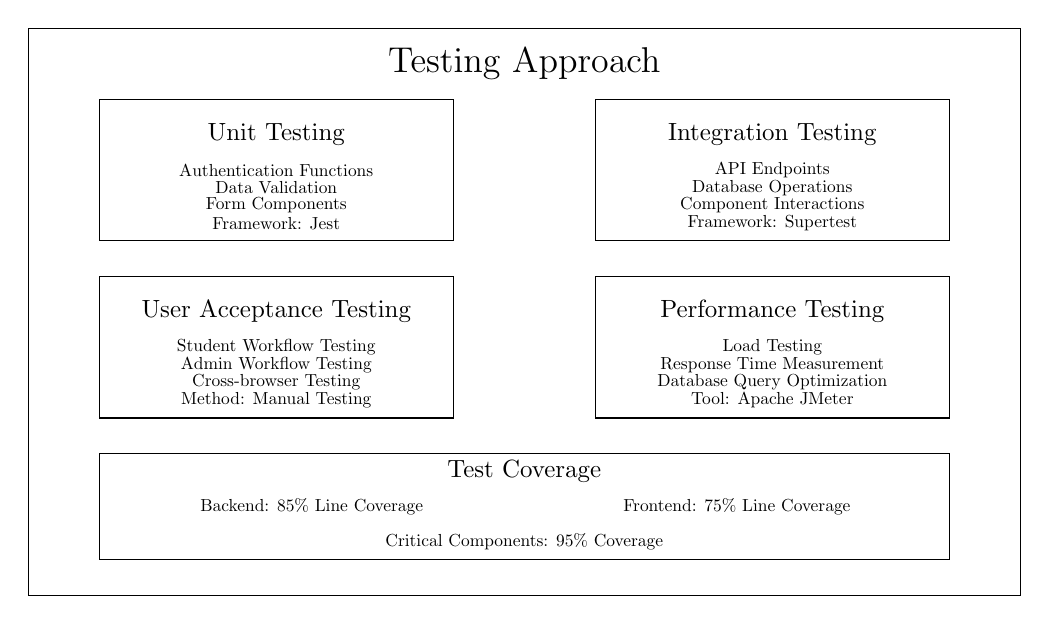
\begin{tikzpicture}[node distance=2cm, scale=0.9, transform shape]
        % Testing approach diagram
        \draw (0,0) rectangle (14,8);
        \draw (7,7.5) node[align=center] {\Large Testing Approach};
        
        % Unit Testing
        \draw (1,7) rectangle (6,5);
        \draw (3.5,6.5) node {Unit Testing};
        \draw (3.5,6) node[scale=0.7] {Authentication Functions};
        \draw (3.5,5.75) node[scale=0.7] {Data Validation};
        \draw (3.5,5.5) node[scale=0.7] {Form Components};
        \draw (3.5,5.25) node[scale=0.7] {Framework: Jest};
        
        % Integration Testing
        \draw (8,7) rectangle (13,5);
        \draw (10.5,6.5) node {Integration Testing};
        \draw (10.5,6) node[scale=0.7] {API Endpoints};
        \draw (10.5,5.75) node[scale=0.7] {Database Operations};
        \draw (10.5,5.5) node[scale=0.7] {Component Interactions};
        \draw (10.5,5.25) node[scale=0.7] {Framework: Supertest};
        
        % User Acceptance Testing
        \draw (1,4.5) rectangle (6,2.5);
        \draw (3.5,4) node {User Acceptance Testing};
        \draw (3.5,3.5) node[scale=0.7] {Student Workflow Testing};
        \draw (3.5,3.25) node[scale=0.7] {Admin Workflow Testing};
        \draw (3.5,3) node[scale=0.7] {Cross-browser Testing};
        \draw (3.5,2.75) node[scale=0.7] {Method: Manual Testing};
        
        % Performance Testing
        \draw (8,4.5) rectangle (13,2.5);
        \draw (10.5,4) node {Performance Testing};
        \draw (10.5,3.5) node[scale=0.7] {Load Testing};
        \draw (10.5,3.25) node[scale=0.7] {Response Time Measurement};
        \draw (10.5,3) node[scale=0.7] {Database Query Optimization};
        \draw (10.5,2.75) node[scale=0.7] {Tool: Apache JMeter};
        
        % Test Coverage
        \draw (1,2) rectangle (13,0.5);
        \draw (7,1.75) node {Test Coverage};
        \draw (4,1.25) node[scale=0.7] {Backend: 85\% Line Coverage};
        \draw (10,1.25) node[scale=0.7] {Frontend: 75\% Line Coverage};
        \draw (7,0.75) node[scale=0.7] {Critical Components: 95\% Coverage};
    \end{tikzpicture}
    \caption{Testing Approach Overview}
    \label{fig:testing-approach}
\end{figure}

\section{Unit Test Example}
Example of a Jest unit test for the authentication controller:

\begin{lstlisting}[language=JavaScript, caption=Authentication Controller Test]
describe('Authentication Controller', () => {
  beforeEach(async () => {
    // Clear test database collections before each test
    await mongoose.connection.collection('admin').deleteMany({});
    await mongoose.connection.collection('ce').deleteMany({});
  });

  describe('Login Function', () => {
    test('should return 400 if username is missing', async () => {
      const response = await request(app)
        .post('/api/auth/login')
        .send({ password: 'password123' });
      
      expect(response.status).toBe(400);
      expect(response.body).toHaveProperty('message');
      expect(response.body.message).toContain('username');
    });

    test('should return 400 if password is missing', async () => {
      const response = await request(app)
        .post('/api/auth/login')
        .send({ username: 'testuser' });
      
      expect(response.status).toBe(400);
      expect(response.body).toHaveProperty('message');
      expect(response.body.message).toContain('password');
    });

    test('should return 401 if user does not exist', async () => {
      const response = await request(app)
        .post('/api/auth/login')
        .send({ username: 'nonexistentuser', password: 'password123' });
      
      expect(response.status).toBe(401);
      expect(response.body).toHaveProperty('message');
      expect(response.body.message).toContain('Invalid credentials');
    });

    test('should return 401 if password is incorrect', async () => {
      // Create a test user first
      const testUser = new CE({
        username: 'testuser',
        name: 'Test User',
        email: 'test@example.com',
        phone: '1234567890',
        registrationNumber: 'R12345',
        branch: 'CE',
        semester: 6,
        yearOfAdmission: 2020,
        cgpa: 8.5
      });
      
      // Set password using Passport local mongoose
      await testUser.setPassword('correctpassword');
      await testUser.save();
      
      // Try to login with wrong password
      const response = await request(app)
        .post('/api/auth/login')
        .send({ username: 'testuser', password: 'wrongpassword' });
      
      expect(response.status).toBe(401);
      expect(response.body).toHaveProperty('message');
      expect(response.body.message).toContain('Invalid credentials');
    });

    test('should return 200 and token for valid credentials', async () => {
      // Create a test user first
      const testUser = new CE({
        username: 'testuser',
        name: 'Test User',
        email: 'test@example.com',
        phone: '1234567890',
        registrationNumber: 'R12345',
        branch: 'CE',
        semester: 6,
        yearOfAdmission: 2020,
        cgpa: 8.5
      });
      
      // Set password using Passport local mongoose
      await testUser.setPassword('correctpassword');
      await testUser.save();
      
      // Try to login with correct password
      const response = await request(app)
        .post('/api/auth/login')
        .send({ username: 'testuser', password: 'correctpassword' });
      
      expect(response.status).toBe(200);
      expect(response.body).toHaveProperty('token');
      expect(response.body).toHaveProperty('user');
      expect(response.body.user.username).toBe('testuser');
      expect(response.body.user.role).toBe('student');
      expect(response.body.user.department).toBe('CE');
      
      // Check that password is not included in response
      expect(response.body.user).not.toHaveProperty('hash');
      expect(response.body.user).not.toHaveProperty('salt');
    });
  });
});
\end{lstlisting}

\chapter{Conclusion and Future Work}

\section{Project Achievements}
The Campus Placement Management System successfully fulfilled its objectives:
\begin{itemize}
    \item Implemented a comprehensive digital platform for managing the entire placement process
    \item Created specialized interfaces for students and administrators with role-based access control
    \item Developed a department-based student organization system for efficient management
    \item Implemented real-time notification framework for timely updates
    \item Created robust application tracking system with comprehensive status management
    \item Designed responsive interface accessible across devices
    \item Ensured security through proper authentication, authorization, and data protection measures
\end{itemize}

\section{Future Enhancements}
Potential future enhancements include:
\begin{itemize}
    \item AI-powered resume scoring and matching system to recommend suitable jobs
    \item Integration with video conferencing tools for online interviews
    \item Mobile application for improved accessibility
    \item Advanced analytics dashboard with predictive metrics
    \item Integration with external job portals for broader opportunities
    \item Blockchain-based verification for academic credentials
    \item Alumni tracking and engagement features
\end{itemize}

\appendix
\chapter{API Documentation}
\chapter{Database Schema Details}
\chapter{User Manual}

\end{document}
